% MDM LaTeX template
% 2021-02-02
% C Morris, using some material from John Hogan and Cameron Hall

% Document class:
\documentclass[10pt,a4paper, twocolumn]{article}
\usepackage[utf8]{inputenc} % Enables direct typing of special characters
\usepackage[english]{babel}
\usepackage{setspace}

% Title, authors, date
\newcommand{\theShortTitle}{A Mathematical Model of a Sphere Falling in Water} 
\newcommand{\theTitle}{{\large MDM3 Introductory Assignment} \\ \theShortTitle}
\newcommand{\theAuthors}{Jake Bowhay}
\title{\theTitle}
\author{\theAuthors}
\date{\today}
\usepackage[title]{appendix}

% Page style
\usepackage[a4paper,top=2cm,bottom=2cm,left=1cm,right=1cm,marginparwidth=2.0cm]{geometry}
%\usepackage[hmarginratio=1:1,top=32mm,columnsep=20pt]{geometry} % Document margins
\usepackage[hang, small,labelfont=bf,up,textfont=it,up]{caption}
\usepackage{booktabs} % Horizontal rules in tables
\usepackage{fancyhdr}
\pagestyle{fancy}
%\headheight=17pt
%\footskip=17pt
\fancyhf{}


% This sets things up so that there is a header with the short version of the title on the left and the page number on the right
\fancyhead[L]{\bfseries \theShortTitle}
\fancyhead[R]{\bfseries \thepage}
\renewcommand{\headrulewidth}{1pt} 

% Bibliography style
\usepackage[
backend=bibtex,
sorting=none
]{biblatex}
\addbibresource{bibliography.bib}

% Line spacing
\usepackage[skip=0.8\baselineskip,indent=0pt]{parskip}

% AMS Packages (maths typesetting)
\usepackage{blkarray}
\usepackage{comment}
\usepackage{amsmath}
\usepackage{amsfonts}
\usepackage{amssymb}
\usepackage{booktabs}

% Importing graphics and defining the graphics path
\usepackage{graphicx}
\graphicspath{{./}{./Figures/}}

% Miscellaneous packages
\usepackage[english]{babel}
\usepackage{csquotes}
\usepackage{color}
\usepackage{lipsum}
\usepackage{hhline}
\usepackage{todonotes}
\usepackage{float}
\usepackage{subcaption}

% Calculus
\newcommand{\de}{\mathrm{d}}
\newcommand{\diff}[2]{\frac{\mathrm{d} #1}{\mathrm{d} #2}}
\newcommand{\ddiff}[2]{\frac{\mathrm{d}^2 #1}{\mathrm{d} #2^2}}
\newcommand{\pdiff}[2]{\frac{\partial #1}{\partial #2}}

% In text
\newcommand{\ie}{\emph{i.e.}}
\newcommand{\eg}{\emph{e.g.}}
\newcommand{\etc}{\emph{etc.}}

% Useful functions
\newcommand{\floor}[1]{\left\lfloor #1 \right\rfloor}
\newcommand{\ceil}[1]{\left\lceil #1 \right\rceil}

% Extra operator names
\newcommand{\erf}{\operatorname{erf}}
\newcommand{\sech}{\operatorname{sech}}
\newcommand{\csch}{\operatorname{csch}}
\newcommand{\signum}{\operatorname{\text{sgn}}}

\usepackage{xcolor,colortbl}
\usepackage[section]{placeins}
\usepackage[none]{hyphenat}

\usepackage{siunitx}

% Hyperlinking within text.
\usepackage{hyperref}
\pdfstringdefDisableCommands{%
	\def\\{}%
}

\hypersetup{
	unicode=true,                 % non-Latin characters in Acrobat bookmarks
	pdftoolbar=true,        % show Acrobat toolbar?
	pdfmenubar=true,       % show Acrobat menu?
	pdffitwindow=true,      % page fit to window when opened
	pdftitle={\theShortTitle},  % title of pdf document
	pdfauthor={\theAuthors},   % author of pdf document
	pdfsubject={},        % subject of the document
	pdfnewwindow=true,      % links in new window
	pdfkeywords={},        % list of keywords
	colorlinks=true,       % false: boxed links; true: colored links
	linkcolor=black,       % color of internal links
	citecolor=black,       % color of links to bibliography
	filecolor=black,       % color of file links
	urlcolor=blue         % color of external links
}


\begin{document}
	
	
	% Create the title and make sure there isn't a page number at the bottom of the page (title is line 12ish)
	\maketitle
	\thispagestyle{empty}
	\setstretch{0.97}
	
	
	\begin{abstract}
		This report considers modelling the velocity of sphere falling through water. A simple model using Stokes' law is presented then compared to experimental data. The Reynolds number is then computed to show this problem falls outside the valid domain of Stokes' law. An improved model of drag is proposed using a drag coefficient. This model is also compared to the experimental data and gives good agreement with the terminal velocity reached. Possible further improvements such as the addition of a virtual weight and the inclusion a Basset force are discussed. 
		
	\end{abstract}
	
	%----------------------------------------------------------------------------------------
	%	Section 1 - Introduction
	%----------------------------------------------------------------------------------------
	
	\section{Introduction}
	\label{sec:intro}
	
	This report seeks to find a mathematical model for a sphere descending in pool of water as shown in \autoref{fig:setup}. The sphere is made from steel and is released from bellow the surface of the water. The model needs to compute the vertical velocity of the sphere as a function of time. The results of the model will be compared to experimental data to validate its performance. The sphere used to generate the experimental data has a mass $m_s=0.11$\si{g} and a radius $R_s=0.15$\si{cm}.
	
	\begin{figure}[!h]
		\centering
		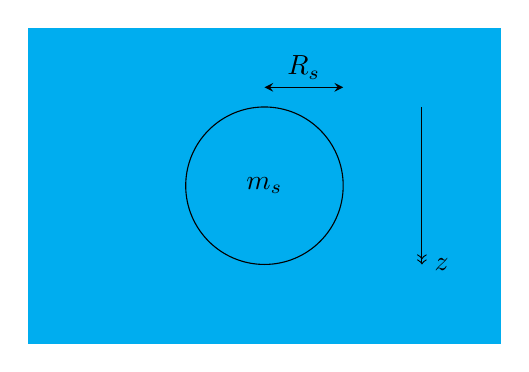
\begin{tikzpicture}
			\filldraw [cyan] (0,0) rectangle (6,4);
			\draw (3,2) circle (1) node {$m_s$};
			\draw [stealth-stealth](3,3.25) -- (4,3.25);
			\draw [->>](5,3) -- (5,1);
			\node[align=center] at (3.5,3.5) {$R_s$};
			\node[align=center] at (5.25,1) {$z$};
		\end{tikzpicture}
		\caption{A sphere of mass $m_s$ and radius $R_s$ descending in water.}
		\label{fig:setup}
	\end{figure}


	
	\section{Stokes' Law Model}
	While descending through the fluid, the sphere is acted upon by three forces: the weight of the sphere, the buoyancy and drag caused by the movement through the water. Newton's second law \cite{Newton1687} dictates that
	
	\begin{equation}
		m_{s}\ddot{z} = F_{\text{Weight}} - F_{\text{Drag}} - F_{\text{Buoyancy}}.
		\label{eq:general}
	\end{equation}
	
	The weight is given by $F_{\text{Weight}} = m_s g$ where $g$ is the acceleration due to gravity. Assuming small Reynolds numbers, the drag force can be modelled Stokes' Law $F_{\text{Drag}} = 6\pi\mu R_s \dot{z} = D \dot{z}$ \cite{stokes1851effect} where $\mu$ is the dynamic viscosity of the fluid. The buoyant force is given by Archimedes' principle $F_{\text{Buoyancy}} = \rho_w g V$ \cite{Archimedes2009} where $\rho_w$ is the density of the fluid and $V = (4/3)\pi R_s^3$ is the volume of the sphere. Substituting these terms into \autoref*{eq:general} and rearranging gives
	
	\begin{equation}
		\ddot{z} + \frac{D}{m_s}\dot{z} = g  - \frac{\rho_w g V}{m_s}.		
		\label{eq:final}
	\end{equation}

	Since the velocity rather than the position is the quantity of interest substituting $v=\dot{z}$ simplifies \autoref{eq:final} into a first order ordinary differential equation (ODE). This ODE can then be solved by multiplying through by the integrating factor $\exp\left((D/m_s)t\right)$, integrating and applying the initial condition $v(0)=0$ as the sphere is released from rest. This gives the solution of the velocity of the sphere as
	
	\begin{equation}
		v(t) = \frac{g}{D}\left(m_s - \rho_w V\right)\left(1 - \exp\left((-\frac{D}{m}t)\right)\right).
	\end{equation}

\bgroup
\def\arraystretch{1.2}
\begin{table}[!h]
	\centering
	\begin{tabular}{|l|l|}
		\hline
		mass of sphere, $m_S$            & 0.11\si{g}   \\ \hline
		radius of sphere, $R_s$          & 0.15\si{\centi\meter}   \\ \hline
		acceleration due to gravity, $g$ & 9.8\si{\meter\per\second}    \\ \hline
		density of water, $\rho_w$       & 997\si{\kilogram\per\meter\cubed}    \\ \hline
		Stokes' drag coefficient, $D$    & 0.0251\si{\gram\per\second} \\ \hline
	\end{tabular}
	\caption{The parameter values used to generate results shown in \autoref{fig:res1}.}
	\label{tab:my-table}
\end{table}
\egroup
	
	As seen in \autoref{fig:res1} when compared to the experimental data the model has poor agreement with the experimental data. Whilst both the model and the data converge to a terminal velocity, this value is an order of magnitude too high. Once source of error is assuming the drag force can be approximated by Stokes' law. Stokes' law is valid for very small Reynolds numbers, $R_e \ll 1$ \cite{white_fluid_2009}, however, computing the Reynolds number $R_e = \rho_w U R_s/\mu$ gives $Re \approx 1000$. This means this scenario is well outside the domain where Stokes' law is valid as the drag is no longer dominated by frictional force but by the complex flows in the wake of the sphere.
	
	\begin{figure}[!h]
		\centering
			\centering
			\includegraphics[width=\linewidth]{../all_comparison}
			\captionof{figure}{Comparison of the Stokes' law model, drag coefficient model and the experimental data.}
			\label{fig:res1}
	\end{figure}
	
	\section{Drag Coefficient Model}
	
	One improvement to \autoref{eq:final} is to consider a non-linear model for the drag force $F_{\text{Drag}} = (1/2)\rho_w \dot{z}^2 C_d A$ where $C_d$ is the coefficient of drag and $A = \pi R_s^2$ is the frontal area of the sphere. This results in
	
	\begin{equation}
		\ddot{z} + \frac{\rho_w C_d A}{2m_s}\dot{z}^2 = g  - \frac{\rho_w g V}{m_s}.		
		\label{eq:finaldrag}
	\end{equation}
	
	Whilst the drag coefficient is a function of the Reynolds and Mach numbers since the range of velocities experienced by the sphere is small $C_d$ is approximated to be constant. A typical value of $C_d$ for a sphere at similar Reynolds numbers to that in the experimental data is $C_d = 0.47$ \cite{drag}.
	
	\autoref{eq:finaldrag} was solved numerically using an Adams–Bashforth type scheme provided by SciPy \cite{2020SciPy-NMeth}. \autoref{fig:res2} shows that the model converges to a terminal velocity that is in agreement with the experimental data. However, the sphere is accelerating too quickly relative to the experimental data suggesting the resistive force is too small.
	
	\begin{figure}[!h]
		\centering
		\includegraphics[width=\linewidth]{../better_comparison}
		\captionof{figure}{Comparison of the drag coefficient model and the experimental data.}
		\label{fig:res2}
	\end{figure}
	
	\section{Further Improvements}
	
	As the sphere accelerates it must move some of the surrounding water. However this added inertia is not accounted for in either model presented as only the inertia of the sphere itself is considered. It is possible to relax this assumption by adding a virtual mass term \cite{white_fluid_2009} which accounts for the inertia required to displace water while the sphere is accelerating.
	
	When the sphere accelerate in the water, the development of a boundary layer is delayed relative to the change in velocity. The Basset force accounts for the delay in boundary layer development \cite{Crowe2011}.
	
	These two additional force would increase the resistive force on sphere therefore lessoning the sphere's initial acceleration. This would help to reduce the error between the model and the experimental.
	
	\section{Conclusion}
	
	In this report two different models have been presented. The first models the drag experienced by the Sphere using Stoke's law. When compared to the experimental data this was shown not to be valid due to the Reynolds number being too high for Stokes' law to be a good model for drag. A second model using a drag coefficient showed much better agreement with the experimental data, with both reaching approximately the same terminal velocity. However the initial acceleration of the sphere is still far greater than the experimental data. This is possibly due the absence of a virtual mass or Basset force which could be included to further improve the model.
	
	%----------------------------------------------------------------------------------------
	%	Bibliography
	%----------------------------------------------------------------------------------------
	
	\printbibliography
	
\end{document}
